\documentclass[tikz,border=4pt]{standalone}
\usepackage{amsmath,amssymb}

\usetikzlibrary{arrows.meta,positioning,automata,shapes,shapes.misc,calc,decorations.pathmorphing,decorations.markings,angles,quotes,patterns,mindmap,matrix,knots,hobby,trees}
\tikzset{->-/.style={decoration={markings, mark=at position 0.5 with {\arrow{Stealth}}}, postaction={decorate}}}
\begin{document}
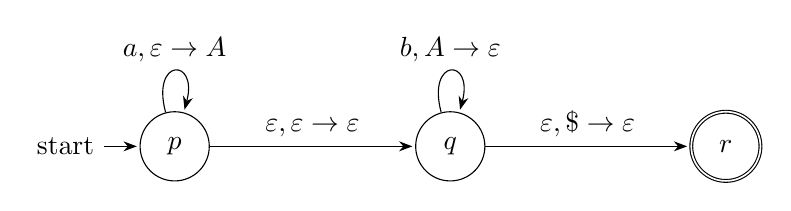
\begin{tikzpicture}[shorten >=1pt, node distance=3.5cm, on grid, auto, >=Stealth]
\node[state, initial] (p) {$p$}; \node[state] (q) [right=of p] {$q$}; \node[state, accepting] (r) [right=of q] {$r$};
\path[->] (p) edge [loop above] node {$a, \varepsilon \to A$} ()
          (p) edge node {$\varepsilon, \varepsilon \to \varepsilon$} (q)
          (q) edge [loop above] node {$b, A \to \varepsilon$} ()
          (q) edge node {$\varepsilon, \$ \to \varepsilon$} (r);
\end{tikzpicture}
\end{document}
